%-----------------------------------------
% To process this file:
%   pdflatex fpp_manual
%-----------------------------------------

%\documentclass{article}
\documentclass{hitec}     % Tutorial overall style

\usepackage{index}
\usepackage{xr}
\usepackage{textgreek}
\usepackage{setspace}
\usepackage{graphicx}
\usepackage{moreverb}    % Defines {listing} environment.
\usepackage{amsmath, amsthm, amssymb, amsbsy, mathtools}
\usepackage{alltt}
\usepackage{rotating}
\usepackage{enumitem}
\usepackage{subcaption}
\usepackage{toc-dcs}    % See toc-dcs.sty file in this directory.
\usepackage{xspace}
%%\usepackage{makeidx}
\usepackage[section]{placeins}   % For preventing floats from floating to end of chapter.
\usepackage{longtable}  % For splitting long vertical tables into pieces
\usepackage{multirow}
\usepackage{booktabs}   % For table layouts
\usepackage{yhmath}     % For widehat
\usepackage{xcolor}      % Needed for listings package.
\usepackage{listings}
\usepackage[T1]{fontenc}   % so _, <, and > print correctly in text.
\usepackage[strings]{underscore}    % to use "_" in text
\usepackage[nottoc,numbib]{tocbibind}   % Makes "References" section show in table of contents
\usepackage[pdftex,colorlinks=true,bookmarksnumbered=true]{hyperref}   % Must be last package!

%----------------------------------------------------------------

\newcommand{\sref}[1]{\S\ref{#1}}
\newcommand{\Sref}[1]{Sec.~\sref{#1}}

\newcommand{\vn}{\begingroup\catcode`\_=11 \catcode`\%=11 \dottcmd}
\newcommand\dottcmd[1]{{\usefont{T1}{lmss}{bx}{n} #1}\endgroup}

\newenvironment{example}
  {\vspace{-3.0ex} \begin{alltt}}
  {\end{alltt} \vspace{-2.5ex}}


\definecolor{light-gray}{gray}{0.95}
\lstset{backgroundcolor=\color{light-gray}}
\lstset{xleftmargin=0cm}
\lstset{framexleftmargin=0.3em}

\lstnewenvironment{Xcode}{}{}

\definecolor{lightcyan}{rgb}{0.88, 1.0, 1.0}
\newcounter{main}
\setcounter{main}{1}
\lstnewenvironment{code}[1][firstnumber=\themain,name=main]
  {\lstset{ %language=haskell,
           %columns=fullflexible,
           columns=fixed,
           basicstyle=\small\ttfamily,
           %numbers=left,
           numberstyle=\tiny\color{gray},
           backgroundcolor=\color{lightcyan},
           #1
          }
}
{\setcounter{main}{\value{lstnumber}}}



\definecolor{backcolor}{rgb}{0.8824,1.0,1.0}   % To match code environment
\lstset{basicstyle = \small, backgroundcolor=\color{backcolor}, escapeinside = {@!}{!@}}

\renewcommand{\textfraction}{0.1}
\renewcommand{\topfraction}{1.0}
\renewcommand{\bottomfraction}{1.0}

\settextfraction{0.9}  % Width of text
\setlength{\parindent}{0pt}
\setlength{\parskip}{1ex}
%\setlength{\textwidth}{6in}
\newcommand{\Section}[1]{\section{#1}\vspace*{-1ex}}

\newenvironment{display}
  {\vspace*{-1.5ex} \begin{alltt}}
  {\end{alltt} \vspace*{-1.0ex}}

\title{The Fully Polymorphic Package Manual}
%\titlehead{adf}

\author{}
\date{
  \parbox{5.5in}{
\includegraphics[width=12cm]{fpp-logo.pdf}} \vspace*{0.5in} \\ 
  Etienne Forest and David Sagan \\ 
  March 25, 2023
}

\begin{document}

\phantomsection
\pdfbookmark[1]{Cover Page}{Cover Page}
\maketitle

\cleardoublepage
\phantomsection
\pdfbookmark[1]{Contents}{Contents}
\tableofcontents

\newpage

%--------------------------------------------------------------------------------------------------------
\Section{Introduction to FPP/PTC}
\label{s:intro}

FPP/PTC is an object oriented, open source, subroutine library for
\begin{itemize}
\item The manipulation and analysis of Taylor series and Taylor maps.
\item Modeling of charged particle beams in accelerators using Taylor maps.
\end{itemize}
FPP/PTC has two parts. The Fully Polymorphic Package (FPP) is the part that deals with Taylor series and maps. FPP is pure math independent1 of any "physics". The Polymorphic Tracking Code (PTC) part of the library deals with the modeling of particle beams and accelerators. PTC contains the "physics" and relies on FPP for producing and manipulating Taylor maps.
This is illustrated in Figure~\ref{f:ptc}. Roughly, FPP can be subdivided into two parts, a Taylor manipulation part for basic manipulations of Taylor series and an analysis part to do things like normal form analysis. PTC uses the Taylor manipulation part of FPP for things like the construction of Taylor maps. Additionally, PTC uses the analysis tools of FPP. A closer look at FPP shows the existence of a Differential Algebra (DA) package within FPP. This package was originally coded by Martin Berz.

This manual covers FPP usage. PTC is covered elsewhere. 

\begin{figure}[tb]
  \centering
  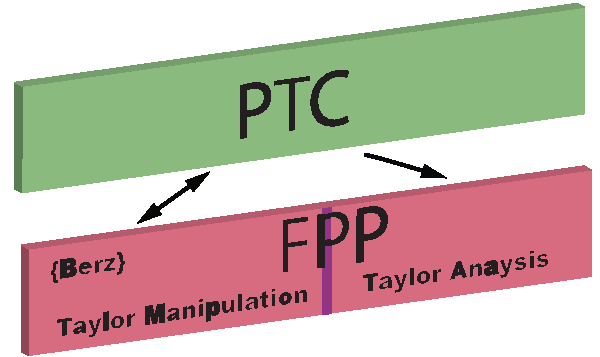
\includegraphics[width=0.8\textwidth]{ptc-fpp.pdf}
  \caption{
The Fully Polymorphic Package (FPP) part of the FPP/PTC library provides manipulation and analysis of Taylor series and maps and the Polymorphic Tracking Code (PTC) part provides the physics from which accelerators can be analyzed.
  }
  \label{f:ptc}
\end{figure}

%--------------------------------------------------------------------------------------------------------
\Section{Where to Obtain FPP/PTC}
\label{s:obtain}

%--------------------------------------------------------------------------------------------------------
\Section{Concepts}
\label{s:concepts}

FPP/PTC is written in Fortran90. It is assumed that the reader has some familiarity with this language. In particular, it is assumed that the reader knows what a \vn{structure} is (roughly corresponding to a \vn{class} in Python or C++) which is also called a \vn{derived type}. Also it is assumed that the reader knows about operator overloading.

FPP/PTC uses double precision numbers. The kind type parameter ``\vn{dp}'' is defined in FPP/PTC to correspond to double precision numbers. For example:
\begin{code}
  real(rp) abc, xyz             ! Declare double precision variables abc and xyz.
  xyz = 3.4_dp * abc / 1e9_dp   ! 3.4_dp and 1e9_dp are double precision numbers.
\end{code}

%--------------------------------------------------------------------------------------------------------
\Section{Taylor and ComplexTaylor Fundamental Types}
\label{s:fundamental}

FPP defines two fundamental structures that are the building blocks of many other structures: \vn{Taylor} and
\vn{complextaylor}. The direct use of either in a tracking program (that is, when doing simulations with PTC) is
discouraged. Rather the \vn{real_8} and \vn{complex_8} structures should be used.

%--------------------------------------------------------------------------------------------------------
\subection{Taylor Type}
\label{s:taylor}

The \vn{taylor} structure overloads the Taylor series of the original real ``DA-Package'' of
Berz. See \sref{sec:real8}. The structure is
\begin{code}
type taylor
   integer i    ! Pointer to Berz
end type taylor
\end{code}
The Berz package uses a positive integer to differentiate different Taylor series and the
\vn{taylor} structure just stores this integer. Since the \vn{real_8} type is similar, and since use
of the \vn{taylor} type is discuraged in favor of \vn{real_8} for tracking simulations, this type will not
be discussed further.

%--------------------------------------------------------------------------------------------------------
\subection{ComplexTaylor Type}
\label{s:taylor}

The \vn{complextaylor} structure stores two Taylor series which represent the real and imaginary parts.
The structure is:
\begin{code}
type complextaylor
   type (taylor) r     ! Real part of complex Taylor series.
   type (taylor) i     ! Imaginary part of complex Taylor series.
end type complextaylor
\end{code}
Since the \vn{complex_8} type is similar, and since use
of the \vn{complextaylor} type is discuraged in favor of \vn{complex_8} for tracking simulations, this type will not
be discussed further.

%--------------------------------------------------------------------------------------------------------
\Section{Real_8 Type}
\label{s:real.8}

FPP defines the \vn{taylor} type (\sref{s:taylor} which holds a Taylor series. Since computations
with Taylor series can be slow, FPP defines ``polymorphic'' type called \vn{real_8}. In general, a
"polymorphic" variable is a variable that can act in different ways depending on the context of the
code. In this case, a \vn{real_8} variable can act as if it were a real number or it can act as if
it were a Taylor series depending upon how it is initialized. An example program will make this clear.
\begin{code}
program real_8_example
use pointer_lattice   ! Read in structure definitions, etc.
implicit none

type (real_8) r8      ! Define a real_8 variable named r8
real(dp) x            ! Define a double precision number

!

nice_taylor_print = .true.    ! Shorten "call print" output
call init (only_2d0, 3, 0)    ! Initialize: #Vars = 2, Order = 3

x = 0.1d0
call alloc(r8)          ! Initialize memory for r8
r8 = x                  ! This will make r8 act as a real

print '(/,a)', 'r8 is now acting as a real:'
call print (r8)

r8 = 0.7d0 + dz_8(1) + 2*dz_8(2)**3 ! Init r8 as a Taylor series
print '(/,a)', 'r8 is now acting as a Taylor series:'
call print(r8)

r8 = r8**4  ! Raise the Taylor series to the 4th power
print '(/,a)', 'This is r8^4:'
call print (r8)

call kill(r8)
end program
\end{code}
The variable \vn{x} is defined as a double precision real number. The line
\begin{example}
  type (real_8) r8
\end{example}
defines \vn{r8} as an instance of a \vn{real_8} variable and the line
\begin{example}
  call alloc(r8)
\end{example}
initializes \vn{r8}. This initialization must be done before \vn{r8} is used. After \vn{r8} is used, any memory that has been allocated for use with \vn{r8} is reclaimed by calling the \vn{kill} routine
\begin{example}
  call kill(r8)
\end{example}
Strictly speaking, the \vn{kill} is not necessary here since \vn{kill} is called at end of the program. However, in a subroutine or function, all local instances of \vn{real_8} variables must be killed otherwise there will be a memory leak.

When \vn{r8} is set to the real number \vn{x} in the line
\begin{example}
    r8 = x
\end{example}
this will cause \vn{r8} to act as a real number. This is verified by printing the value of \vn{r8} in the lines
\begin{example}
  print *, 'r8 is now acting as a real:'
  call print (r8)
\end{example}
The output is just a single real number indicating that \vn{r8} is acting as a real:
\begin{example}
  r8 is now acting as a real:'
  0.100000000000000
\end{example}
Notice that the \vn{print} statement uses the Fortran intrinsic print function while the \vn{call print} statement uses the overloaded print subroutine defined by \vn{FPP}.

When \vn{r8} is set to a Taylor series in the line
\begin{example}
  r8 = 0.7d0 + dz_8(1) + 2*dz_8(2)**3 ! Init r8 as a Taylor series
\end{example}
this will cause \vn{r8} to act as a Taylor series. To understand how this initialization works, first consider the initialization of FPP/PTC which was done by the line
\begin{example1}
  call init (only_2d0, 3, 0)  ! Initialize FPP/PTC. #Vars = 2, Order = 3
\end{example1}
The first argument, \vn{only_2d0},  configured FPP/PTC to construct any Taylor series as a function of two phase space variables. These two variables will be called $z_1$ and $z_2$ here. The second argument, \vn{3}, gives the order at which the Taylor series is truncated to. That is, after this initialization, all Taylor series $t$ will be of the form
\begin{equation}
    t = \sum_{i,j}^{0 \le i+j \le 3} C_{ij} \, z_1^i \, z_2^j
\end{equation}
In the above initialization of \vn{r8}, \vn{dz_8(1)} represents the variable $z_1$ and \vn{dz_8(2)} represents the variable $z_2$. Thus \vn{r8} is initialized to the Taylor series
\begin{equation}
    t = 0.7 + z_1 + 2 \, z_2^3
\end{equation}
This is confirmed by printing \vn{r8} after it has been set via the lines
\begin{example}
  print *, 'r8 is now acting as a Taylor series:'
  call print(r8)
\end{example}
The output is:
\begin{example}
  r8 is now acting as a Taylor series:
  Properties, NO =    3, NV =    2, INA =   21
   *********************************************

     0  0.7000000000000000       0  0
     1   1.000000000000000       1  0
     3   2.000000000000000       0  3
\end{example}
Each line in the above output, after the line with the asterisks, represents one term in the Taylor series. The general form for printing a Taylor term is:
\begin{example}
  <term-order>   <term-coefficient>    <z1-exponent>  <z2-exponent>
\end{example}
The <term-order> is the order of the term. That is, the sum of the exponents. For example, the last line in the above printout is
\begin{example}
   3   2.000000000000000       0  3
\end{example}
and this line represents the term $2 \, z_1^0 \, z_2^3$. 

Once \vn{r8} has been initialized, it can be used in expressions. Thus the line
\begin{example}
  r8 = r8**4  ! Raise the Taylor series to the 4th power
\end{example}
raises \vn{r8} to the 4th power and puts the result back into \vn{r8}. This is confirmed by the final print which produces
\begin{example}
  This is r8^4:
  Properties, NO =    3, NV =    2, INA =   23
  *********************************************

    0  0.2400999999999999       0  0
    1   1.372000000000000       1  0
    2   2.940000000000000       2  0
    3   2.800000000000000       3  0
    3   2.743999999999999       0  3
\end{example}
Notice that the map has been truncated so that no term has an order higher than 3 as expected. Expressions using \vn{real_8} variables involve overloaded operators as discussed in section \sec{sec:over}.

%--------------------------------------------------------------
\subsection{Real\_8 Under the Hood}\label{sec:real8}

The particulars of how the \vn{real_8} structure is defined are generally not of interest to the general user. But it is instructive to take a quick look. In the \vn{FPP} code the \vn{real_8} structure is defined as:
\begin{example1}
  TYPE REAL_8
     TYPE (TAYLOR) T      !  USED IF TAYLOR
     REAL(DP) R           !    USED IF REAL
     INTEGER KIND  !  0,1,2,3 (1=REAL,2=TAYLOR,3=TAYLOR KNOB)
     INTEGER I   !   USED FOR KNOBS AND SPECIAL KIND=0
     REAL(DP) S   !   SCALING FOR KNOBS AND SPECIAL KIND=0
     LOGICAL(LP) :: ALLOC  1 IF TAYLOR IS ALLOCATED IN DA-PACKAGE
  END TYPE REAL_8
\end{example1}
The \vn{t} component of the structure is of type \vn{taylor} and is used if a \vn{real_8} variable is acting as a Taylor series. The \vn{r} component is used if a \vn{real_8} variable is acting as a real number. The \vn{kind} component is an integer that sets the behavior of a \vn{real_8} variable. Besides behaving as \vn{real} or a \vn{Taylor series}, a \vn{real_8} variable may behave as a "\vn{knob}" which will be explained later.

The \vn{real_8} structure contains a component of type \vn{taylor}. The definition of the taylor structure is
\begin{example1}
  TYPE TAYLOR
     INTEGER I       !  integer I is a pointer in old da-package of Berz
  END TYPE TAYLOR
\end{example1}
The component \vn{i} is a pointer to the differential algebra package of Berz that is contained in FPP. The details of how a Taylor series is stored in the structure is not important here. What is important is that this structure can be used to hold a Taylor series.

The reason for hiding a Taylor series under the hood is to defer its use to running time. We really do not know in a tracking code like PTC when the user will need a Taylor series and even what the parameters of that series might be: phase space, if so how many (2,4,6,?), and parameters such as quadrupole strengths which are taken from the huge set of magnets present in the system.

%-------------------------------------------------------------------
\subsubsection{Type \protect\vn{real_8}}  \label{sec:real8code}

The \vn{real_8} type was discussed in Sec.~\sref{s:concepts} and Sec.~\sref{sec:real8}.
This type is the most important type if you write a tracking code of respectable length.  Imagine that your code tracks in one degree of freedom (1-d-f). Then you will push two phase space variables through your magnets, let us call them ${\bf z}=(z_1,z_2)$. These variables will denote  the position and the tangent of an angle in our little example.  If it is your  intention to always extract a Taylor series around a special orbit, then  it would suffice to declare as \vn{taylor} only the phase space variables ${\bf z}=(z_1,z_2)$ and any temporary variables the code might used during its calculations. 

But what if we want to have a Taylor map that also depends upon some parameter or parameters of the lattice. For example, a map can include quadrupole strengths as independent variables in the maps. Such variables are called ``\vn{knobs}.'' Since this is a user decision, it is best if the code decides at execution time using the type \vn{real_8}.
As an example, consider the code \vn{z_why_polymorphism.f90}:

\begin{code}
program my_small_code_real_8
use polymorphic_complextaylor
implicit none
type(real_8) :: z(2)  
real(dp) :: z0(2) = [0, 0]  ! special orbit
type(reaL_8)  :: L , B, K_q , K_s 
integer :: nd = 1 , no = 2 , np = 0, ip
longprint = .false.         ! Shorten "call print" output
! nd = number of degrees of freedom
! no =  order of Taylor series
! Number of extra variables beyond 2*nd

call alloc(z)
call alloc( L , B, K_q , K_s )
np=0
print * , "Give  L and parameter ordinality (0 if not a parameter)"
read(5,*) L%r , ip
np=np+ip
call make_it_knob(L,ip);  np=np+ip;
print * , "Give  B  and parameter ordinality (0 if not a parameter)"
read(5,*) K_q%r , ip
print * , "Give  K_q and parameter ordinality (0 if not a parameter)"
read(5,*) K_q%r , ip
call make_it_knob(K_q,ip);  np=np+ip;
print * , "Give  K_s and parameter ordinality (0 if not a parameter)"
read(5,*) K_s%r , ip
call make_it_knob(K_s,ip); np=np+ip;
print * , "The order of the Taylor series ?"
read(5,*) no

call init(no,nd,np) ! Initializes TPSA 

z(1)=z0(1) + dz_8(1) ! <--- Taylor monomial z_1 added
z(2)=z0(2) + dz_8(2) ! <--- Taylor monomial z_2 added

call track(z)

call print(z)

contains

subroutine track(z)
implicit none
type(real_8) :: z(2) 
 z(1)=z(1)+L*z(2) 
 z(2)=z(2)-B-K_q*z(1)-K_s*z(1)**2 
end subroutine track

end program my_small_code_real_8
\end{code}

In this little code, there is one drift of length \vn{L} followed by a multipole kick that contains a dipole of strength \vn{B}, a quadrupole of strength \vn{K_q} and a sextupole of strength \vn{K_s}. We run the code ignoring the parameters:

\begin{example1}
 Give  L and parameter ordinality (0 if not a parameter)
1 0
 Give  B  and parameter ordinality (0 if not a parameter)
0 0
 Give  K_q and parameter ordinality (0 if not a parameter)
.1 0
 Give  K_s and parameter ordinality (0 if not a parameter)
0 0
 The order of the Taylor series ?
2

 Properties, NO =    2, NV =    2, INA =   20
 *********************************************

   1   1.000000000000000       1  0
   1   1.000000000000000       0  1


 Properties, NO =    2, NV =    2, INA =   21
 *********************************************

   1 -0.1000000000000000       1  0
   1  0.9000000000000000       0  1
\end{example1}

This little program produces Taylor series to second order in the phase space variables ${\bf z}=(z_1,z_2)$ similar to the programs \vn{Transport} and \vn{Marylie}.
However, we can now require that the multipole strengths be variables of the Taylor series without recompiling the program. In this example, we make the quadrupole strength the third variable of TPSA:  $K_q=0.1 + dz_3$.

\begin{example2}
 Give  L and parameter ordinality (0 if not a parameter)
1 0
 Give  B  and parameter ordinality (0 if not a parameter)
0 0
 Give  K_q and parameter ordinality (0 if not a parameter)
.1 1
 Give  K_s and parameter ordinality (0 if not a parameter)
0 0
 The order of the Taylor series ?
2

 Properties, NO =    2, NV =    3, INA =   22
 *********************************************

   1   1.000000000000000       1  0  0
   1   1.000000000000000       0  1  0


 Properties, NO =    2, NV =    3, INA =   23
 *********************************************

   1 -0.1000000000000000       1  0  0
   1  0.9000000000000000       0  1  0
   2  -1.000000000000000       1  0  1
   2  -1.000000000000000       0  1  1
\end{example2}

Again, we must emphasize that while it would have been easy here to use the type \vn{taylor} for all the variables, it is totally unfeasible in a real tracking code to either recompile the code or allow all parameters of the systems to be Taylor series. This is why typical matrix\footnote{This is not true of Berz's COSY INFINITY which handles variable memory of TPSA within its own internal language.} codes, not using TPSA, are limited to a small set of Taylor variables, usually the six phase space variables.

So in summary a \vn{real_8} polymorph can be as mentioned in \sec{sec:real8}:

\begin{enumerate}
 \item A real number
 \item a Taylor series with real coefficients (\vn{taylor})
 \item a knob which is a simple temporary Taylor series activated only if needed
\end{enumerate}


Notes:

calling init again wipes out existing Taylor series. (Does is wipe out universial taylor?)

\end{document}


